\documentclass[fleqn,10pt]{wlscirep}
\usepackage{subcaption} % subcation of figures, Fig.8 uses it with a, b, c 
\usepackage[nodayofweek]{datetime}
\usepackage{graphicx} % used to include pictures like JPG format fang 20150805
\usepackage{color}
\usepackage{tikz} % use the tikz package for coordination
\usepackage{tikz-3dplot}  % plot 3D coordination system by tikz pakcage
\usepackage{geometry}
\geometry{left=2.0cm,right=1.9cm,top=1.9cm,bottom=2.0cm}
\linespread{1.4}  % 1 is for single row spacing, 1.2 is one and half, 1.6 is double spacing

\title{Notes for ray trancing}

\author[1,*]{Yue-Wen Fang}
\affil[1]{Key Laboratory of Polar Materials and Devices, Ministry of Education, Department of Electronic Engineering, East China Normal University, Shanghai, 200241, China}
\affil[*]{fyuewen@gmail.com or fyuewen@protonmail.ch}
%\affil[+]{these authors contributed equally to this work}
\newcommand*{\PV}{POV-Ray}
\newcommand*{\DF}{Definition in English}
\newcommand*{\LAOSTO}{LaAlO$_3$$\slash$SrTiO$_3$}
\newcommand*{\LAO}{LaAlO$_3$}
\newcommand*{\STO}{SrTiO$_3$}
%\keywords{Keyword1, Keyword2, Keyword3}

\begin{abstract}
Ray-tracing is a significant method for design. Here, the author presents his notes for leaning the software POV-Ray v3.7 based on his own knowledge and understanding.
\end{abstract}

\begin{document}
\flushbottom
\maketitle
% * <john.hammersley@gmail.com> 2015-02-09T12:07:31.197Z:
%
%  Click the title above to edit the author information and abstract
%
\thispagestyle{empty}

\renewcommand{\thesubsection}{\arabic{subsection}}  %rename the stype of subsection. you can use roman and alpha to replace arabic

\section*{Getting started}
This part will guide you how to generate your first image by \PV.
\subsection{The first scene}
\subsubsection{The coordinate system}
The \PV sticks with a so called "left-handed system", in which we point our \textbf{thumb} in the direction of \emph{\textbf{x}}, the \textbf{index} finger in the direction of \emph{\textbf{y}} and the \textbf{middle} finger in the positive \emph{\textbf{z}} direction.\\

%\begin{figure}[htbp]
%\centering
%\includegraphics[width=20pc,clip]{FIG1}
%\caption{\label{fig:wide} A left-handed coordinates system in \PV.}
%\label{fig:FIG1}
%\end{figure}
%%%%%%%%%%%%%%%%%%
\begin{figure}[htbp]
\centering
%%You must note that in tikz package, a right-handed coordinate system is used
\tdplotsetmaincoords{60}{120}

% customized coordinate system
\let\raarotold\raarot \let\rbarotold\rbarot
\let\rabrotold\rabrot \let\rbbrotold\rbbrot
\let\racrotold\racrot \let\rbcrotold\rbcrot

\let\raarot\racrotold \let\rbarot\rbcrotold
\let\rabrot\rabrotold \let\rbbrot\rbbrotold
\let\racrot\raarotold \let\rbcrot\rbarotold

\begin{tikzpicture}[tdplot_main_coords]

  % axes
  \draw[thick,->] (0,0,0) -- ( 5,0,0) node[anchor=south]{$y$};
  \draw[thick,->] (0,0,0) -- ( 0,5,0) node[anchor=west]{$x$};
  \draw[thick,->] (0,0,0) -- ( 0,0,5) node[anchor=north east]{$-z$};
  \draw[thick]    (0,0,0) -- ( 0,-2,0);
  \draw[thick,->] (0,0,0) -- ( 0,0,-5) node[anchor=south west]{$z$};

  % vector 1
  \pgfmathsetmacro{\ax}{5}
  \pgfmathsetmacro{\ay}{5}
  \pgfmathsetmacro{\az}{2}
  \draw[very thick,->,red] (0,0,0) -- (\ax,\ay,\az) node[anchor=west]{};

   % vector 2
  \pgfmathsetmacro{\bx}{1}
  \pgfmathsetmacro{\by}{0}
  \pgfmathsetmacro{\bz}{-2}
  \draw[very thick,->,blue] (2,0,3) node[anchor=north]{camera} -- (\bx,\by,\bz) node[anchor=north]{look\_at};

   % vector 3 (projection)
  \pgfmathsetmacro{\cx}{\ax*1.2}
  \pgfmathsetmacro{\cy}{0}
  \pgfmathsetmacro{\cz}{\az*1.2}
  \draw[very thick,green] (0,0,0) -- (\cx,\cy,\cz);

   % dashed lines
%  \draw[dashed,gray] (\ax,\ay,\az) -- (\ax,\ay,0);
  \draw[dashed,gray] (\ax,\ay,\az) -- (\ax,0,\az);
  \draw[dashed,gray] (\ax,\ay,\az) -- (0,\ay,\az);
%  \draw[dashed,gray] (\ax,0,0) -- (\ax,\ay,0) -- (0,\ay,0);
  \draw[dashed,gray] (\ax,0,0) -- (\ax,0,\az) -- (0,0,\az);
  \draw[dashed,gray] (0,0,\az) -- (0,\ay,\az) -- (0,\ay,0);

  % arcs
  \tdplotdefinepoints(0,0,0)(\ax,\ay,\az)(\bx,\by,\bz)
  \tdplotdrawpolytopearc[<->]{2}{anchor=north west}{$\theta$}
  \tdplotdefinepoints(0,0,0)(0,0,1)(\bx,\by,\bz)
  \tdplotdrawpolytopearc[<->]{3}{anchor=north}{$\beta$}
  \tdplotdefinepoints(0,0,0)(1,0,0)(\cx,\cy,\cz)
  \tdplotdrawpolytopearc[<->]{4}{anchor=north}{$\phi$}

\end{tikzpicture}

\caption{\label{fig:wide} A left-handed coordinates system in \PV.}
\label{fig:FIG1}
\end{figure}
%%%%%%%%%%%%%%%%%
\noindent This coordinate is plotted by a package called \textbf{tikz} which supports Latex. Note that in \textbf{tikz} package, a right-handed coordinate system is used, so when you are plotting, you have to take care of the conversion between the left-handed and right-handed coordinates.
%%%%%%%%%%%%%%%%%


\subsubsection{Adding standard include files}
Create a file called demo.pov. The \PV-v3.7 in windows has a built-in text editor which is easy to use. However, in \textbf{Linux}, I prefer using \textbf{Vim}.\\
\newline
After creating the demo.pov, type the following text,\\
\textcolor[rgb]{0.2,0.1,1}{\emph{\#}include "colors.inc"}\ \ \     // The include files contain \\
\textcolor[rgb]{0.2,0.1,1}{\emph{\#}include "stones.inc"}\ \ \     // pre-defined scene elements\\
where '//' is the comment character. Line-1 reads in defections for various useful colors and Line-2 reads in a collection of stone textures (\DF: the surface of a material, the structure of a woven fabric). \PV provides many interesting include files as the following lines show:\\
\textcolor[rgb]{0.2,0.1,1}{\emph{\#}include "texture.inc"}\ \ \     // The include files contain\\
\textcolor[rgb]{0.2,0.1,1}{\emph{\#}include "shapes.inc"}\ \ \     // pre-defined scene elements\\
\textcolor[rgb]{0.2,0.1,1}{\emph{\#}include "glass.inc"}\ \ \     // pre-defined scene elements\\
\textcolor[rgb]{0.2,0.1,1}{\emph{\#}include "metals.inc"}\ \ \     // pre-defined scene elements\\
\textcolor[rgb]{0.2,0.1,1}{\emph{\#}include "woods.inc"}\ \ \     // pre-defined scene elements\\
it should be noted that \textbf{do not include overmany include files because some of them come with \PV{} are quite large. For saving parsing time and memory, we'd better include what we really need.} In the following examples we just include "colors.inc" and "stones.inc". Sometimes we may need as many include files as possible, some include files may themselves contain include files, but we are limited to declaring includes (nested only ten levels deep). The include files (with suffix .Inc) should be in the current path or the library paths (in Linux, we can set them in .bashrc). Usually in windows, the include files are automatically installed in the \emph{\textbf{include}} directory of the installation directory of \PV.

\subsubsection{Adding a camera}
The \textbf{camera} statement describes where and how the camera sees the scene. It uses \emph{x}-,\emph{y}- and \emph{z}-coordinates to indicate the position of the camera and what part of the scene it is pointing at. The coordinates in the 2D space is denoted by a three-part vector written as $\langle$x, y, z$\rangle$. Here, commas are used to separate the values of x, y and z.\\
\newline
Here is a simple example.\\
\textcolor[rgb]{0.2,0.1,1}{camera\{}  \\
\textcolor[rgb]{0.2,0.1,1}{  location $\langle$0, 2, -3$\rangle$}  \\
\textcolor[rgb]{0.2,0.1,1}{  look$\_$at $\langle$0, 1, 2$\rangle$}  \\
\textcolor[rgb]{0.2,0.1,1}{\}} \\
\newline
Briefly, \textcolor[rgb]{0.2,0.1,1}{  location $\langle$0, 2, -3$\rangle$}  places the camera up 2 units and back 3 units from the center of the ray-tracing universe which is at \textcolor[rgb]{0.2,0.1,1}{$\langle$0, 0, 0$\rangle$}. \textcolor[rgb]{0.2,0.1,1}{look$\_$at $\langle$0, 1, 2$\rangle$} \textbf{rotates} the camera to point at the coordinates \textcolor[rgb]{0.2,0.1,1}{$\langle$0, 1, 2$\rangle$}. This make it 5 units in  front of and 1 unit lower than the camera which can be seen from Fig. \ref{fig:FIG1} \textbf{The \textcolor[rgb]{0.2,0.1,1}{look$\_$at} point should be the center of attention of our image }

\subsubsection{Describeing an object}
Now that the camera is set up, let's place a sphere into the cene by input the following lines:\\
\textcolor[rgb]{0.2,0.1,1}{sphere \{} \\
\textcolor[rgb]{0.2,0.1,1}{\ \ $\langle$0, 1, 2$\rangle$, 2}    \ \ \ \ \  //center of sphere, raidus\\
\textcolor[rgb]{0.2,0.1,1}{\ \ texture \{} \\
\textcolor[rgb]{0.2,0.1,1}{\ \ \ \ pigment \{color Yellow\}} \\
\textcolor[rgb]{0.2,0.1,1}{\ \ \}} \\
\textcolor[rgb]{0.2,0.1,1}{\ \}} \\
The vector specifies the center of sphere. In this example the x coordinate is zero so it is \textbf{centered left and right}. It is 1 unit up from the origin and z = 2 shows the center of the sphere is 5 units in front of the camera (z = -3). After the center vector is a comma followed by the \textbf{radius}.

\subsubsection{Adding texture to an object}
Now we need define the appearance using \textbf{texture} which specifies color, bumpiness (\DF: uneven, rough) and finish properties (\DF: to put a particular surface texture on (wood, cloth, etc)) of an object. In the following example we will speccify the color only. The parameter \textbf{pigment} in \PV{} determines how the color of the object appears.\\
\textcolor[rgb]{0.2,0.1,1}{ color red 1.0 green 0.8 blue 0.8} \\
This example gives a nice shade of pink. Actually, a shortcut notation can be used to remove the superfluous (\DF: exceeding what is sufficient or required), as shown in the following.
\textcolor[rgb]{0.2,0.1,1}{ color rgb $\langle$1.0, 0.8, 0.8$\rangle$} \\
or \\
\textcolor[rgb]{0.2,0.1,1}{ color $\langle$1.0, 0.8, 0.8$\rangle$} \\

\subsubsection{Defining a light source}
We have created an object with specific texture, so we need a light to illuminate it by adding the line \\
\textcolor[rgb]{0.2,0.1,1}{light$\_$source {$\langle$2, 4, -3$\rangle$ color \textbf{W}hite}} \\
to the scene file to get our first complete \PV scene file as shown below.\\
\textcolor[rgb]{0.2,0.1,1}{\emph{\#}include "colors.inc"}\ \ \     // The include files contain \\
\textcolor[rgb]{0.2,0.1,1}{background \{color \textbf{C}yan\}}\ \ \ // defining color of background \\
\textcolor[rgb]{0.2,0.1,1}{camera\{}  \\
\textcolor[rgb]{0.2,0.1,1}{  location $\langle$0, 2, -3$\rangle$}  \\
\textcolor[rgb]{0.2,0.1,1}{  look$\_$at $\langle$0, 1, 2$\rangle$}  \\
\textcolor[rgb]{0.2,0.1,1}{\}} \\
\textcolor[rgb]{0.2,0.1,1}{sphere \{} \\
\textcolor[rgb]{0.2,0.1,1}{\ \ $\langle$0, 1, 2$\rangle$, 2}    \ \ \ \ \  //center of sphere, raidus\\
\textcolor[rgb]{0.2,0.1,1}{\ \ texture \{} \\
\textcolor[rgb]{0.2,0.1,1}{\ \ \ \ pigment \{color Yellow\}} \\
\textcolor[rgb]{0.2,0.1,1}{\ \ \}} \\
\textcolor[rgb]{0.2,0.1,1}{\ \}} \\
\textcolor[rgb]{0.2,0.1,1}{light$\_$source \{$\langle$2, 20, -3$\rangle$ color \textbf{W}hite\}} \\
\newline
The produced picture is shown in Fig. \ref{fig:FIG2}. If your hardware such as monitor or GPU is not good, you may cannot get a high color or true color displaying in your monitor, but details of your operations all all written to the image file regardless of the type of display.\\

Though the scene we just traced is not quite "state of the art" but we will have to start with basics before we soon get to much more fascinating features and scenes.

\begin{figure}[htbp]
\centering
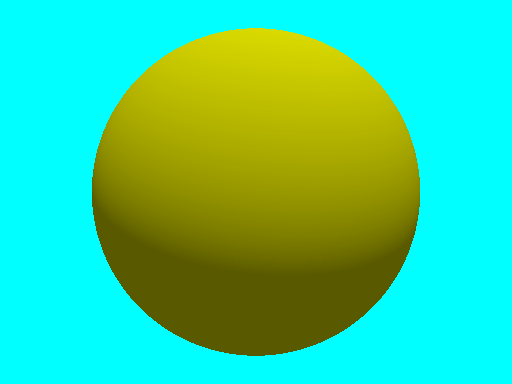
\includegraphics[width=20pc,clip]{FIG2}
\caption{The first basic scene generated by \PV.}
\label{fig:FIG2}
\end{figure}

\subsection{Basic shapes}
So far we have just used the sphere shape. The following sections will describe how to use other simple objects as a replacement for the sphere used above.
\subsubsection{Box object}

\begin{figure}[htbp]
\centering
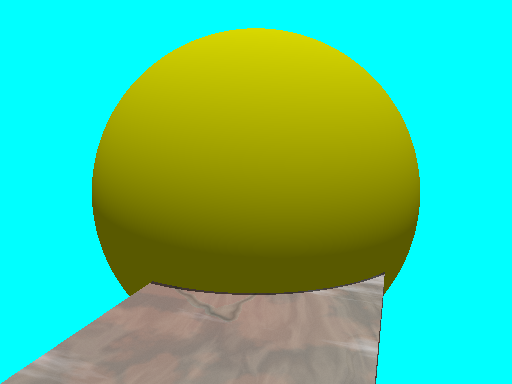
\includegraphics[width=20pc,clip]{FIG3}
\caption{A sphere and a box generated by \PV.}
\label{fig:FIG3}
\end{figure}

The \textbf{box} is one of the common objects used. We try this example in comnination of the previous sphere:\\
\textcolor[rgb]{0.2,0.1,1}{box \{} \\
\textcolor[rgb]{0.2,0.1,1}{\ \ $\langle$-1, 0, -1$\rangle$}\ \ \ // Near lower left corner \\
\textcolor[rgb]{0.2,0.1,1}{\ \ $\langle$1, 0.5, 3$\rangle$}\ \ \ // Far upper right corner \\
\textcolor[rgb]{0.2,0.1,1}{\ \ texture\{} \\
\textcolor[rgb]{0.2,0.1,1}{\ \ \ \ T\_Stone25}\ \ \ //Pre-defined from stones.inc \\
\textcolor[rgb]{0.2,0.1,1}{\ \ \ \ scale 4}\ \ \ //Scale by the same amount in all directions \\
\textcolor[rgb]{0.2,0.1,1}{\ \ \}} \\
\textcolor[rgb]{0.2,0.1,1}{\ \ rotate y*20}\ \ \ //Equivalent to "rotate $\langle$0, 20, 0$\rangle$" \\
\textcolor[rgb]{0.2,0.1,1}{\ \}} \\



We see in the above example a box is defined by specifying the 3D coordinates of its opposite coiners (any two opposie corners may be used). We can then rotate them to any angle (e.g. rotate x*100 as shown in Fig. \ref{fig:FIG3} which combines the box with the sphere leaving the source of light and camera no variations).\\
\subsubsection{Cone object}

\begin{figure}[htbp]
\centering
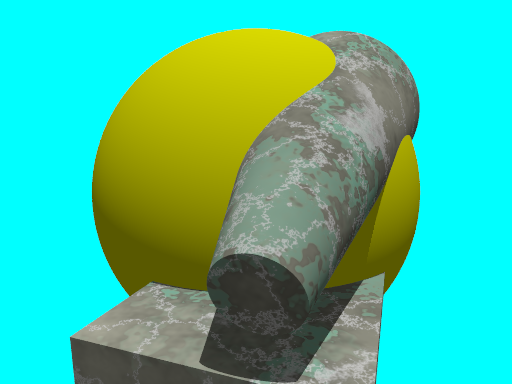
\includegraphics[width=20pc,clip]{FIG4}
\caption{A sphere, a cone and a box generated by \PV.}
\label{fig:FIG4}
\end{figure}

We can use the following lines to show a \textbf{cone}:\\
\textcolor[rgb]{0.2,0.1,1}
{
cone\{ \\
\ \ $\langle$0, 1, -1$\rangle$, 0.3 \\
\ \ $\langle$1, 2, 2$\rangle$, 1.0  \\
\ \ \ texture \{T\_Stone25 scale 4\} \\
\ \ \}
}\\
Here, Line-2 defines one center and the radius, and Line-3 defines another center and the corresponding radius. The produced scene is shown in Fig. \ref{fig:FIG4}.
\newline
\textbf{\{This part is finished in  26 November, 2015\}}
\subsubsection{Cylinder object}
cylinder can be defined like this:\\
\textcolor[rgb]{0.2,0.1,1}
{
cylinder \{ \\
\ \ $\langle$0, 2, 2$\rangle$ \\
\ \ $\langle$1, 0, -3$\rangle$ \\
\ \ 0.5 \\
\ \ open \\
\ \ texture \{T\_Stone25 scale 4\} \\
\}\\
}\\
%\newline
Line-2 and Line-3 define centers of each side, Line-4 is the radius of the cylinder. \textbf{open} meands "Remove and caps"\\

Figure \ref{fig:FIG5} including a sphere and a cylinder is produced by the following codes:\\
\noindent \textcolor[rgb]{0.2,0.1,1}{\emph{\#}include "colors.inc"}\\
\textcolor[rgb]{0.2,0.1,1}{\emph{\#}include "stones.inc"}\\
\textcolor[rgb]{0.2,0.1,1}{background \{color Cyan\}} \\
\textcolor[rgb]{0.2,0.1,1}{\ \ \ \ camera\{ } \\
\textcolor[rgb]{0.2,0.1,1}{ location $\langle$0, 2, -3$\rangle$ } \\
\textcolor[rgb]{0.2,0.1,1}{ look\_at $\langle$0, 1, 2$\rangle$  } \\
\textcolor[rgb]{0.2,0.1,1}{ \}  } \\

\textcolor[rgb]{0.2,0.1,1}{ sphere \{ } \\
\textcolor[rgb]{0.2,0.1,1}{ $\langle$0, 1, 2$\rangle$, 1 } \\
//center of sphere, raidus \\
\textcolor[rgb]{0.2,0.1,1}{texture \{ } \\
\textcolor[rgb]{0.2,0.1,1}{ pigment \{color Yellow\} } \\
\textcolor[rgb]{0.2,0.1,1}{ \} } \\
\textcolor[rgb]{0.2,0.1,1}{ \} } \\

\textcolor[rgb]{0.2,0.1,1}{ cylinder\{ } \\
\textcolor[rgb]{0.2,0.1,1}{ $\langle$0, 3, 2$\rangle$ } \\
\textcolor[rgb]{0.2,0.1,1}{ $\langle$0, -1, 2$\rangle$ } \\
\textcolor[rgb]{0.2,0.1,1}{ 0.4 } \\
\textcolor[rgb]{0.2,0.1,1}{ open } \\
\textcolor[rgb]{0.2,0.1,1}{ texture \{T\_Stone25 scale 4\} } \\
\textcolor[rgb]{0.2,0.1,1}{ \} } \\
\textcolor[rgb]{0.2,0.1,1}{ light\_source \{$\langle$2, 20, -3$\rangle$ color White\} }  \\

\begin{figure}[htbp]
\centering
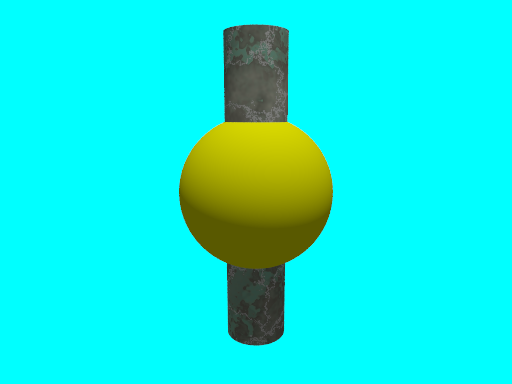
\includegraphics[width=20pc,clip]{FIG5}
\caption{A sphere, a cylinder generated by \PV.}
\label{fig:FIG5}
\end{figure}

\subsubsection{Plane object}
Now let us try to add a "\textbf{plane} object to Fig. \ref{fig:FIG5}, the new figure is shown in Fig. \ref{fig:FIG6}. This figure shows we have built a nice "checkered floor" with only several lines as following:\\
\textcolor[rgb]{0.2,0.1,1}
{
plane \{ $\langle$0, 1, 0$\rangle$, -1\\
pigment \{  \\
checker color Red, color Blue  \\
\}  \\
\}  \\
} \\
\newline
The object defined here is an infinite plane. $\langle$0, 1, 0$\rangle$ defines the surface normal of the plane. The number afterward (-1) is the distance that the plane is displaced along the normal from the origin. We use -1 so that the sphere and the cylinder are on the "floor". Here even though we do not use a \textbf{texture} statement there is an implied (\DF: not directly expressed) texture here. It is tiresome if we continually (\DF: recurring frequently) typing statements that are nested like \textbf{texture \{pigment\}}, so \PV let us leave out the \textbf{texture} under many circumstances. In general we only need the texture block surrounding a texture identifier (e.g. T\_Stone25 in the previous examples), or when creating layered textures which will be covered later. \\
\newline
Besides, in the example, pigment uses the checker color pattern and specifies that the two colors red and blue should be used. Because the vectors $\langle$1, 0, 0$\rangle$, $\langle$0, 1, 0$\rangle$ and $\langle$0, 0, 1$\rangle$ are used frequently thus \PV has provided us three built-in vector identifiers x, y and z respectively that can be used as a shorthand. Thus the plane could be defines as:\\
\textcolor[rgb]{0.2,0.1,1}
{
plane \{ \\
y, -1  \\
pigment\{...\}  \\
\}  \\
}

\begin{figure}[htbp]
\centering
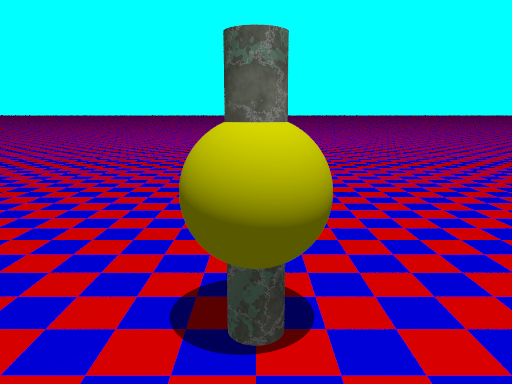
\includegraphics[width=20pc,clip]{FIG6}
\caption{A sphere and a cylinder on a plane.}
\label{fig:FIG6}
\end{figure}

Look at Fig. \ref{fig:FIG6}, a precise, sharp shadow is created by the ray-tracer in \PV. In the real word, penumbral (\DF: the point or area in which light and shade blend) or "soft" shadows are often seen. Later we will learn how to use extended light sources to soften the shadows.


\subsubsection{Torus object}
A torus is a ring-shaped surface that can be thought as a donut or an inner-tube. It is a kind of useful Constructive Solid Geometry (CSG) so \PV has adopted this 4th order quartic polynominal as a primitive shape. In \PV, the major and minor radius is defines as shown in Fig. \ref{fig:FIG7}a. The syntax for a torus is so simple that it makes it a very easy shape to work with once we learn what the two float values mean. Now, let's produce it!\\
\newline
We create a file called \textbf{tordemo.pov} and edit it as follows:\\
{\color{blue}
\{\#\}include "colors.inc"   \\
camera \{   \\
\ \ location $\langle$0, .1, -25$\rangle$   \\
\ \ look\_at 0   \\
\ \ angle 30    \\
\}   \\
background \{color Gray50\} \ \ // to make the torus easy to see   \\
light\_source \{$\langle$300, 300, -1000$\rangle$ White\}   \\
torus \{   \\
\ \ 4, 1    \ \ //major and minor radius   \\
\ \ rotate -90*x \ \ // so we can see it from the top  \\
\ \ pigment \{ Green \} \\
\}  \\
}\\

\begin{figure}[htbp]
\centering
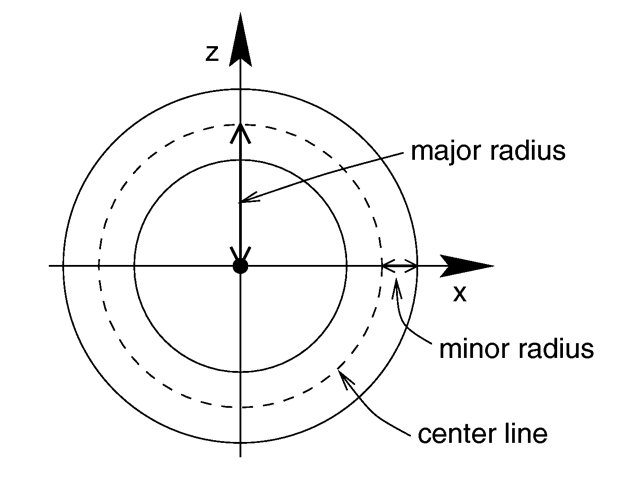
\includegraphics[width=20pc,clip]{FIG7a}
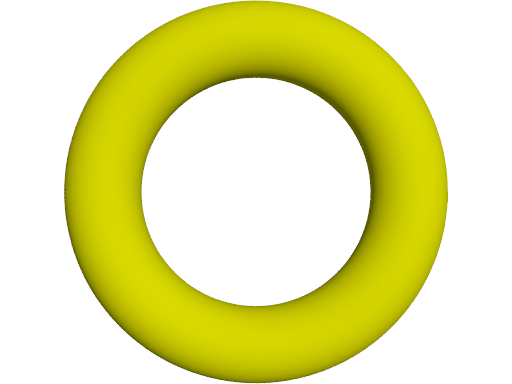
\includegraphics[width=16pc,clip]{FIG7b}
\caption{a. The definition of major and minor raidus. b. A donut-like torus. To make the same background of a and b, I used a white background instead of Gray50}
\label{fig:FIG7}
\end{figure}

You can see a nice-looking "donut" in Fig. \ref{fig:FIG7}b, changing radius can turn the "donut" into "hula-loop"-like (major 4,minor 0.3) torus. However, using such simple syntax we cannot do much else. Let us see... \\
\newline
Tori are very useful CSB, and we can try a little experiment with it. We make a \textbf{difference} of a torus and a box:\\
{\color{blue}
difference \{
\ \ torus \{ \\
\ \ \ 4, 1  \\
\ \ \ rotate -90*x \ \ // so we can see it from the top  \\
\ \ \}  \\
\ \ box \{$\langle$-5, -5, -1$\rangle$, $\langle$5, 0, 1$\rangle$\}  \\
 pigment \{Yellow\}  \\
\}  \\ 
}\\
Interesting... a half-torus as shown in Fig. \ref{fig:FIG8a}.


\textbf{\{This part is finished in  27 November, 2015.\}}\\
\newline
\begin{figure}
\begin{subfigure}{0.31\textwidth}

\includegraphics[width=\linewidth]{FIG8a}
\caption{A half-torus} \label{fig:FIG8a}
\end{subfigure}
\hspace*{\fill} % separation between the subfigures
\begin{subfigure}{0.31\textwidth}

\includegraphics[width=\linewidth]{FIG8b}
\caption{Two half-tori} \label{fig:FIG8b}
\end{subfigure}
\hspace*{\fill} % separation between the subfigures
\begin{subfigure}{0.31\textwidth}
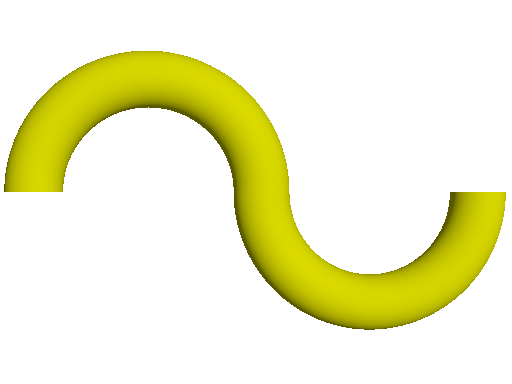
\includegraphics[width=\linewidth]{FIG8c}
\caption{Same to b but with a optimized camera} \label{fig:FIG8c}
\end{subfigure}
\caption{\textbf{Torus} object} \label{}
\end{figure}
In the previous part, we have produced a half-torus, now we add another one flipped the other way. Only, let's declare the original half-torus and the necessary transformations so we can use them again: \\
{\color{blue}
\#declare Half\_Torus = difference \{  \\
\ \ torus \{ \\
\ \ \ 4, 1  \\
\ \ \ rotate -90*x \ \ // so we can see it from the top  \\
\ \ \}  \\
\ \ box \{$\langle$-5, -5, -1$\rangle$, $\langle$5, 0, 1$\rangle$\}  \\
\ \ pigment \{ Yellow \}  \\
\}  \\
\#declare Flip\_It\_Over = 180*x;  \\
\#declear Torus\_Translate = 8;\ \ // twice the major radius
}\\
Fig. \ref{fig:FIG8b} shows two connected half-tori. Note that we do not modify the parameters of background, camera and light source. One might find that we cannot see the whole scene of Fig. \ref{fig:FIG8b}, it requires us to make a minor fix of the \textbf{location} and \textbf{camera}, for example, look\_at $\langle$3.8, 0, 0$\rangle$ and location $\langle$0, .1, -34$\rangle$ can display more, as shown in Fig. \ref{fig:FIG8c}.\\
\newline
\textbf{union} is very useful as we have used just now, we can use it to make more torus like this:\\
{\color{blue}
\{\#\}include "colors.inc"   \\
camera \{   \\
\ \ location $\langle$0, .1, -34$\rangle$   \\
\ \ look\_at $\langle$3., 0, 0$\rangle$   \\
\ \ angle 30    \\
\}   \\
background \{color White\} \ \ // to make the torus easy to see   \\
light\_source \{$\langle$300, 300, -1000$\rangle$ White\}   \\
}\\
{\color{blue}
\#declare Half\_Torus = difference \{  \\
\ \ torus \{ \\
\ \ \ 4, 1  \\
\ \ \ rotate -90*x \ \ // so we can see it from the top  \\
\ \ \}  \\
\ \ box \{$\langle$-5, -5, -1$\rangle$, $\langle$5, 0, 1$\rangle$\}  \\
\ \ pigment \{ Yellow \}  \\
\}  \\
\#declare Flip\_It\_Over = 180*x;  \\
\#declear Torus\_Translate = 8;\ \ // twice the major radius
}\\
{\color{blue}
union\{ \\
object \{Half\_Torus\}  \\
object \{Half\_Torus  \\
\ \ rotate Flip\_It\_Over \\
\ \ translate x*Torus\_Translate  \\
\} \\
object \{Half\_Torus  \\
\ \ translate x*Torus\_Translate*2  \\
\}  \\
object \{Half\_Torus  \\
\ \ rotate Flip\_It\_Over  \\
\ \ translate x*Torus\_Translate*3  \\
\}  \\
object \{Half\_Torus  \\
\ \ rotate Flip\_It\_Over  \\
\ \ translate -x*Torus\_Translate  \\
\}  \\
object \{Half\_Torus  \\
\ \ translate -x*Torus\_Translate*2  \\
\}  \\
object \{Half\_Torus  \\
\ \ rotate Flip\_It\_Over  \\  
\ \ translate -x*Torus\_Translate*3 \\
\} \\
object \{Half\_Torus  \\
\ \ translate -x*Torus\_Translate*4  \\
\} \\
rotate y*65  \\
translate z*30  \\
\}  \\
}\\
The new scene is plotted in Fig. \ref{fig:FIG9}. We can see a cool, undulating, snake-like something-or-other. Neato (\DF: wonderful).

\begin{figure}[htbp]
\centering
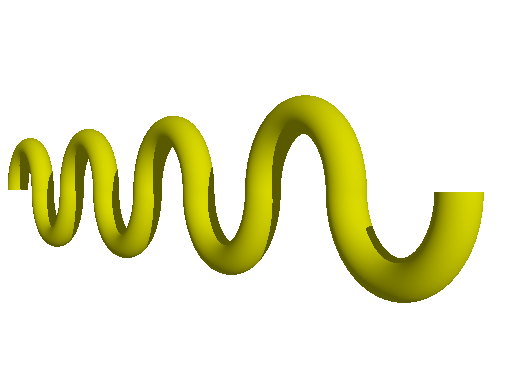
\includegraphics[width=20pc,clip]{FIG9}
\caption{A undulating, snake-like object}
\label{fig:FIG9}
\end{figure}
\noindent Actually we can model something useful like a chain. Thinking about it for a moment, we realize that a single link of chain is composed of two half tori and two cylinders. We create a new file chain.pov. We can use the same camera, background, light source and declared objects and transformations as we used in tordemo.pov:\\
{\color{blue}
\{\#\}include "colors.inc"   \\
camera \{   \\
\ \ location $\langle$0, .1, -34$\rangle$   \\
\ \ look\_at $\langle$3., 0, 0$\rangle$   \\
\ \ angle 30    \\
\}   \\
background \{color White\} \ \ // to make the torus easy to see   \\
light\_source \{$\langle$300, 300, -1000$\rangle$ White\}   \\
}\\
{\color{blue}
\#declare Half\_Torus = difference \{  \\
\ \ torus \{ \\
\ \ \ 4, 1  \\
\ \ \ rotate -90*x \ \ // so we can see it from the top  \\
\ \ \}  \\
\ \ box \{$\langle$-5, -5, -1$\rangle$, $\langle$5, 0, 1$\rangle$\}  \\
\ \ pigment \{ Yellow \}  \\
\}  \\
\#declare Flip\_It\_Over = 180*x;  \\
\#declear Torus\_Translate = 8;\ \ // twice the major radius
}\\
Based on this, we can add a complete torus of two half tori:\\
{\color{blue}
union\{ \\
object \{Half\_Torus\}  \\
object \{Half\_Torus  \\
\ \ rotate Flip\_It\_Over \\
\} \\
}\\
This may seem like a wasteful way to make a complete torus, but we are really going to move each half apart to make room for the cylinders. First we add the declared cylinder \textbf{before} the union:\\
{\color{blue}
\#declare Chain\_Segment = cylinder \{  \\
 $\langle$0, 4, 0$\rangle$,  $\langle$0, -4, 0$\rangle$, 1\\
 pigment \{Blue\}  \\
\}  \\
}\\
\newline
We then add two \textbf{Chain\_Segments} to the union and translate them so that they line up with the minor radius of the torus on each side.\\
{\color{blue}
union\{ \\
 object \{Half\_Torus\}  \\
 object \{Half\_Torus\ rotate Flip\_It\_Over\}  \\
 object \{Chain\_Segments translate x*Torus\_Translate/2\}  \\
 object \{Chain\_Segments translate -x*Torus\_Translate/2\}  \\
\}  \\
}\\
%\newline
Before pushing forward, we can produce this scene in Fig. \ref{fig:FIG10a} first. Then we can translate the two half tori along +y and -y so that the clipped (\DF: neatly cut) ends of the cylinders. This distance is equal to half of the previously declared Torus\_Translate:\\
{\color{blue}
union\{  \\
\ \ object\{  \\
\ \ \ Half\_Torus  \\
\ \ \ translate y*Torus\_Translate/2  \\
\}  \\
\ \ object\{  \\
\ \ \ Half\_Torus\ rotate Flip\_It\_Over  \\
\ \ \ translate -y*Torus\_Translate/2  \\
\}  \\
\ \ object\{  \\
\ \ \ Chain\_Segment  \\
\ \ \ translate x*Torus\_Translate/2 \\
\}  \\
\ \ object\{  \\
\ \ \ Chain\_Segment  \\
\ \ \ translate -x*Torus\_Translate/2  \\
\}\\
\}\\
}\\
Yew, Fig. \ref{fig:FIG10b} is what we just generate using \PV. It's cool. In order to get whole scene, I move the camera location to farther (location $\langle$0, .1, -45$\rangle$) and voila, the updated scene is displayed in Fig. \ref{fig:FIG10c}

\begin{figure}
\begin{subfigure}{0.31\textwidth}
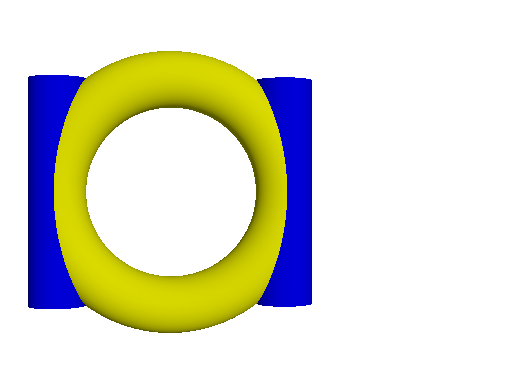
\includegraphics[width=\linewidth]{FIG10a}
\caption{A torus and two cylinders} \label{fig:FIG10a}
\end{subfigure}
\hspace*{\fill} % separation between the subfigures
\begin{subfigure}{0.31\textwidth}
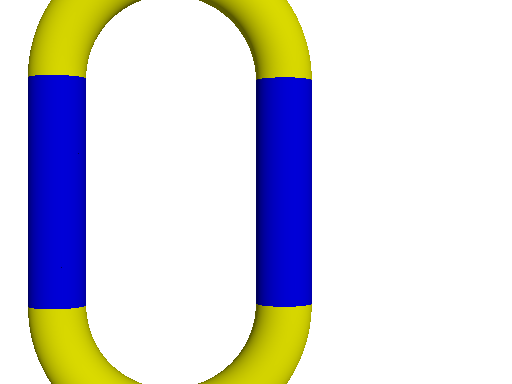
\includegraphics[width=\linewidth]{FIG10b}
\caption{A single link} \label{fig:FIG10b}
\end{subfigure}
\hspace*{\fill} % separation between the subfigures
\begin{subfigure}{0.31\textwidth}
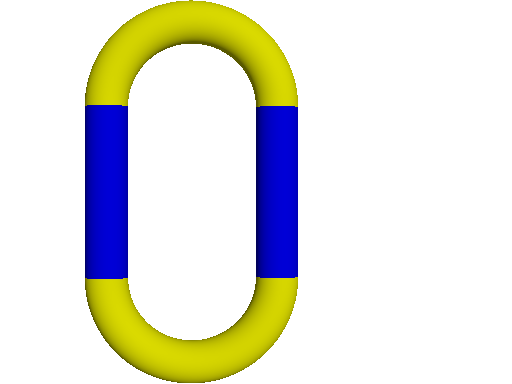
\includegraphics[width=\linewidth]{FIG10c}
\caption{A single link seen from a farther camera} \label{fig:FIG10c}
\end{subfigure}
\caption{\textbf{Torus} Construction a link from torus and cylinders.} \label{}
\end{figure}
Yes, we have got a single link. But we are not done yet! I used two colors in the link to let you have a deep insight of how \PV works with these objects. Now we need use a nice metallic color instead. \\
\textbf{\{This part is finished in  29 November, 2015\}}\\
First,


\subsubsection*{Torus object}


Example text under a subsection. Bulleted lists may be used where appropriate, e.g.

\begin{itemize}
\item First item
\item Second item
\end{itemize}

\section*{Discussion}

The Discussion should be succinct and must not contain subheadings.

\section*{Methods}
\textbf{First-principles calculations.}

%\bibliography{povray}

%\noindent LaTeX formats citations and references automatically using the bibliography records in your .bib file, which you can edit via the project menu. Use the cite command for an inline citation..

\section*{Acknowledgements}



\section*{Author contributions}


\section*{Additional information}

%To include, in this order: \textbf{Accession codes} (where applicable);
\textbf{Supplementary Information} accompanies this paper at http://www.nature.com/srep \\
\newline
\textbf{Competing financial interests:} The authors declare no competing financial interests.



\begin{table}[ht]
\centering
\begin{tabular}{|l|l|l|}
\hline
Condition & n & p \\
\hline
A & 5 & 0.1 \\
\hline
B & 10 & 0.01 \\
\hline
\end{tabular}
\caption{\label{tab:example}Legend (350 words max). Example legend text.}
\end{table}

Figures and tables can be referenced in LaTeX using the ref command, e.g. Table \ref{tab:example}.

\end{document}